\documentclass[11pt]{article}

%%%%%%%%%%%%%%Include Packages%%%%%%%%%%%%%%%%%%%%%%%%%%
\usepackage{xcolor}
\usepackage{mathtools}
\usepackage[a4paper, total={6in, 8in}, margin=1.25in]{geometry}
\usepackage{amsmath}
\usepackage{amssymb}
\usepackage{paralist}
\usepackage{rsfso}
\usepackage{amsthm}
\usepackage{wasysym}
\usepackage[inline]{enumitem}   
\usepackage{hyperref}
\usepackage{tocloft}
\usepackage{titlesec}
\usepackage{colortbl}
\usepackage{wrapfig}
\usepackage{pdfpages}
%%%%%%%%%%%%%%%%%%%%%%%%%%%%%%%%%%%%%%%%%%%%%%%%%%%%%%%%



\begin{document}
\begin{wrapfigure}[9]{r}{0.3\textwidth}
  \begin{center}
  \vspace{-15pt}
    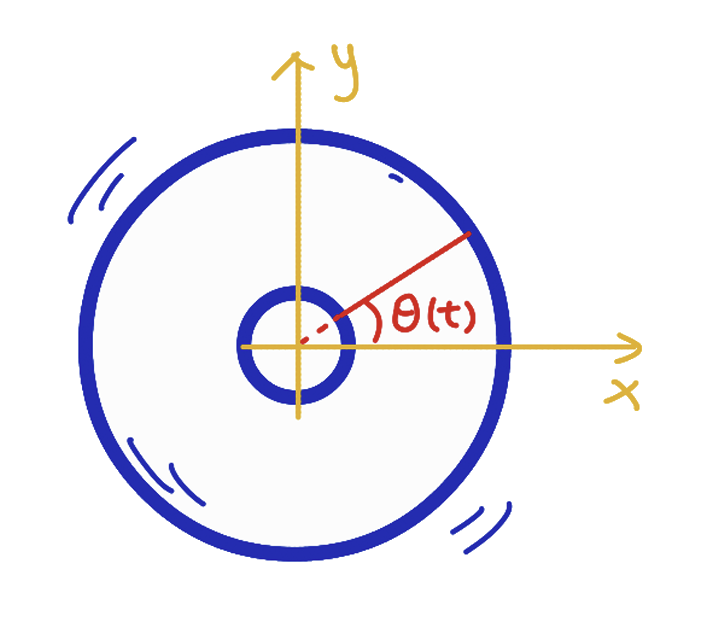
\includegraphics[scale=0.19]{disk}
  \end{center}
\end{wrapfigure}
\Large \noindent \textbf{Physics 1A Discussion (Week 8)}\\
\normalsize
Department of Physics and Astronomy, UCLA\\
\noindent\rule{8cm}{0.4pt}\\
\textbf{Problem 1:} Consider a spinning disk. Jinyan drew a line on the disk, and the line is making a time-dependent angle $\theta(t) = a + bt -ct^3$ with respect to the $x$-axis as shown, where $a$, $b$, and $c$ are constants, and $t$ is measured in seconds. When $t = 0$ seconds, it is found that $\theta = \pi/4$ and the angular velocity of the disk is $2.00$ rad/s. When $t = 1.50$ seconds, it is found that the angular acceleration of the disk is $1.25$ rad/s$^2$. \\

\noindent (a) Find $a$, $b$, and $c$ based on the given information, including their units.\\

\noindent (b) Find the angular acceleration of the disk when $\theta= \pi/4$ rad.\\

%\noindent (c) Find the angle $\theta$ and the angular velocity when the angular acceleration of the disk is $3.50$ rad/s$^2$.

\newpage
\noindent\textbf{Problem 2:}
Show that (by computing the integral) the moment of inertia of a solid rod of length $L$, radius $R$, and mass $M$, rotating about an axis through one end of the rod, is 
\begin{align*}
I = \int |\vec{r}_\perp|^2 \, dm = \frac{ML^2}{3} + \frac{MR^2}{4}\,.
\end{align*}
Assume that the rod has uniform mass density. Here $\vec{r}_\perp$ is a vector perpendicular to the axis of rotation, extending from a point on the rotation axis to a point $\vec{r}$ in the solid rod, and the integral is over the entire rod. 
\begin{center}
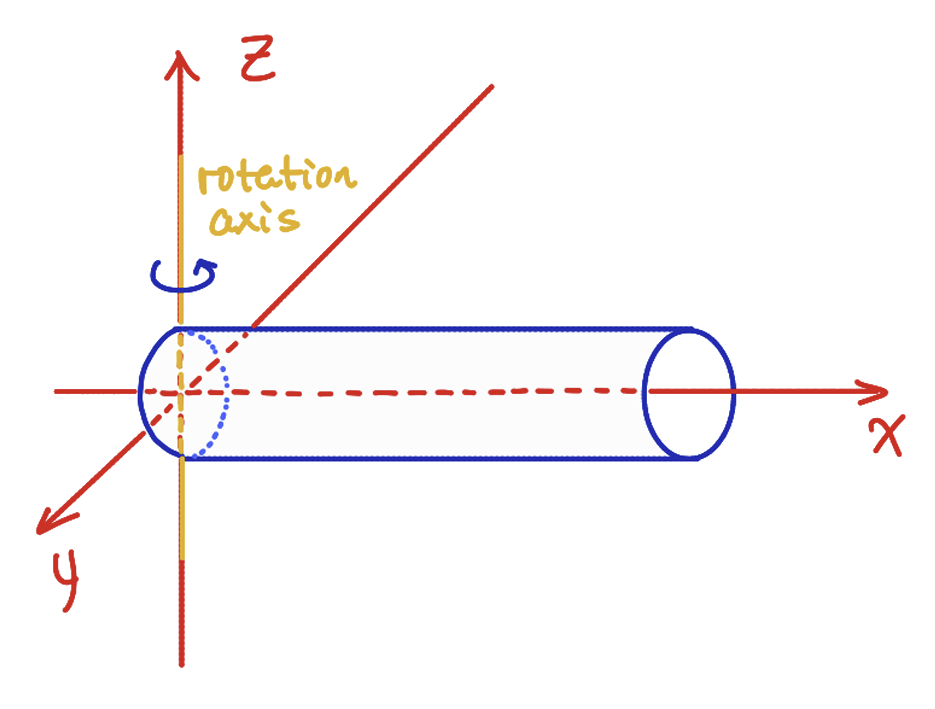
\includegraphics[scale=0.19]{rod}
\end{center}


\newpage
\textbf{Problem 1}: Part (a) is an initial value problem (or boundary value problem when talking about differential equations in general). Here the angular velocity is defined as taking the first derivative of $\theta$ with respect to time, denoted as $\dot{\theta}$. The angular acceleration is defined as taking the second derivative of $\theta$ with respect to time, denoted as $\ddot{\theta}$. \\

To find $a$, $b$, and $c$, we need to utilize the information about the disk at $t = 0$ and $t = 2$ given in the problem. There are exactly three data points given, and we need to use all three of them to solve for the values of the three variables $a$, $b$, and $c$. Namely: the first one is $\theta(t=0) = \pi/4$, which gives
\begin{align*}
\frac{\pi}{4}=\theta(t=0) = a\,;
\end{align*}
the second one is $\dot{\theta}(t=0) = 2$, which gives
\begin{align*}
2 =\frac{d\theta}{dt}|_{t = 0} = b - 3ct^2 |_{t = 0} = b\,;
\end{align*}
and the last one is $\ddot{\theta}(t=1.5) = 1.25$, which gives
\begin{align*}
1.25 = \frac{d^2 \theta}{dt^2}|_{t = 1.5} = -6ct|_{t=1.5}\,,
\end{align*}
and thus $c = -0.139$. Now for the unit of each quantity, we know that $\theta$ is measured in rad, so $a$ should also be measured in rad because $a$ and $\theta$ should have the same physical dimension. On the other hand, $bt$ and $\theta$ have the same physical dimension, so $b$ is measured in rad per second, same as angular velocity. Lastly, $\theta$ and $ct^3$ have the same physical dimension, so $c$ is measured in rad per second cubed (rad/s$^3$). \\

Part (b) is finding the angular acceleration of the disk when $\theta = \pi/4$, first we want to find the time when the disk gets to $\theta = \pi/4$, so we set
\begin{align*}
\frac{\pi}{4} = \frac{\pi}{4} + 2t +0.139 t^3\,,
\end{align*}
from which we get 
\begin{align*}
t = 0 \,\text{seconds }\quad \text{ or } \quad t=\sqrt{-\frac{2}{0.139}}\,\text{seconds}\,.
\end{align*}
Time cannot be imaginary, so we are only interested in the $t = 0$ seconds case. At time $t = 0$, the acceleration of the disk is 
\begin{align*}
\frac{d^2 \theta}{dt^2}|_{t = 0} = -6ct|_{t=0} = 0\,\text{rad/s$^2$}\,.
\end{align*}

%Now for part (c), we want to first find the time when the disk gets to $\ddot{\theta}= 3.5$ rad/s$^2$, that is 
%\begin{align*}
%3.5 = \frac{d^2 \theta}{dt^2}|_t = (-6) \cdot (-0.139)\cdot t\,,
%\end{align*}
%and thus we find $t = 4.20$ seconds, from which we can calculate
%\begin{align*}
%\theta(t = 4.2) = 19.5\,\text{rad}\,,\qquad
%\frac{d\theta}{dt}|_{t=4.2} = 9.36\,\text{rad/s}\,.
%\end{align*}


\textbf{Problem 2}: We want to evaluate the following integral:
\begin{align*}
I = \int_{\text{rod}} r_{\perp}^2 dm = 
\int\int\int_{\text{rod}} r_{\perp}^2 \rho \, dx\, dy\, dz\,,
\end{align*}
where I have used the change of variable
\begin{align*}
dm = \frac{dm}{dV} \, dV = \frac{dm}{dV} \, dx\, dy\, dz = \rho \, dx\, dy\, dz\,.
\end{align*}
It is mentioned in the problem that the mass density $\rho$ is uniform, that is $\rho$ is a constant, independent on the spatial position, and we can write
\begin{align*}
\rho = \frac{M}{\text{volume of the rod}}= \frac{M}{\pi R^2 L}\,.
\end{align*}
Anyway, $\rho$ is just a constant, and we can pull it out of the integral, thus the integral becomes
\begin{align*}
I = \rho \int \int \int_{\text{rod}} r_{\perp}^2 \, dx\, dy\, dz\,.
\end{align*}
Now we want to figure out what $\vec{r}_{\perp}$ is. By definition, it is a vector measured from the rotation axis (the $z$-axis in this case) to a point in the rod, being perpendicular to the rotation axis. Thus, if we have a point $\vec{r} = (x,y,z)$ in the rod, then the corresponding $\vec{r}_{\perp}$ is the component of $\vec{r}$ that is perpendicular to the rotation axis, so
\begin{align*}
\vec{r}_{\perp} = (x,y,0)\,,\qquad
|\vec{r}_{\perp}|^2 = x^2 + y^2\,.
\end{align*}
Now\begin{align*}
I = \rho \int \int \int_{\text{rod}} (x^2+y^2) \, dx\, dy\, dz
=\rho \int_{-R}^R\int_{-\sqrt{R^2 - z^2}}^{\sqrt{R^2 - z^2}}
 \int_{0}^L(x^2 + y^2)\, dx\, dy\,dz\,.
\end{align*}
A direct computation is given here,
\begin{align*}
I &= 
\rho \int_{-R}^R\int_{-\sqrt{R^2 - z^2}}^{\sqrt{R^2 - z^2}}
\left[ \frac{x^3}{3} + y^2 x\right]_{x=0}^{x=L}\, dy\, dz
\\
&=\rho \int_{-R}^R\int_{-\sqrt{R^2 - z^2}}^{\sqrt{R^2 - z^2}}
\left( \frac{L^3}{3} + y^2 L\right)
\, dy\,dz\\
&= \rho \int_{-R}^R 
\left[
\frac{L^3y}{3} + \frac{y^3L}{3}
\right]_{y=-\sqrt{R^2 - z^2}}^{\sqrt{R^2 - z^2}}\, dz\\
&=\rho \int_{-R}^R \left(\frac{2L^3}{3}\left( R^2 - z^2\right)^{1/2} + \frac{2L}{3}\left( R^2 - z^2\right)^{3/2}\right)\, dz\\
&= \rho \left(
\frac{\pi L^3 R^2}{3} + \frac{\pi L R^4}{4}
\right)\tag{*}\\
&=\frac{ML^2}{3} + \frac{MR^2}{4}\,.
\end{align*}
Here I used online integral calculator to brute force calculating the $dz$ integral because I was lazy. It is also possible to carry out the $dz$ integral with a change of variable 
\begin{align*}
z = R\sin(\theta)\,,\qquad\text{s.t. }dz = R\cos(\theta) \, d\theta\,.
\end{align*}
However, we can also use symmetry to do the $dy\, dz$ double integral. In this case, we are integrating over a circular disk on the $yz$-plane, 
\begin{align*}
\int\int_{\text{disk}} \left( \frac{L^3}{3} + y^2 L\right) \, dy\, dz = \frac{L^3}{3}\int\int_{disk}\, dy\, dz + L \int\int_{\text{disk}}y^2\, dy\, dz \,.
\end{align*}
The first term is just
\begin{align*}
\frac{L^3}{3} \cdot (\text{area of the disk}) = \frac{ \pi L^3 R^2}{3}
\end{align*}
which is exactly the first term we obtained in (*). The second term in the disk integral can be evaluated using the symmetry 
\begin{align*}
\int\int_{\text{disk}}y^2\, dy\, dz =
\int\int_{\text{disk}}z^2\, dy\, dz\,.
\end{align*}
Here $y^2 + z^2 = r^2$ where $r$ is the radial polar coordinate on the disk, thus we use polar coordinate integration to compute
\begin{align*}
\int\int_{\text{disk}}r^2 \, r\, dr\, d\theta = \int_0^{2\pi}\int_0^R r^3 \, dr\, d\theta = \frac{\pi R^4}{2}\,.
\end{align*}
Thus we see
\begin{align*}
L\int\int_{\text{disk}}y^2\, dy\, dz = \frac{L}{2}\int\int_{\text{disk}}(y^2+z^2)\, dy\, dz = \frac{L}{2}\int\int_{\text{disk}}r^2 \, r\, dr\, d\theta = \frac{\pi L R^4}{4}\,,
\end{align*}
which is exactly the second term we expect to see in the previous calculation from (*). \\

\noindent\rule{8cm}{0.4pt}\\
Now, what if the radius of the base of the cylinder is approaching zero, that is $R \sim 0$, from the calculation above, we expect to see
\begin{align*}
I = \frac{ML^2}{3}\,.
\end{align*}
Let us verify this: This setup is sometimes referred to the ``thin rod," where the radius of the rod is negligible and we can essentially treat the rod as a one-dimensional object (like a string), so the corresponding integral for computing $I$ will be a one-dimensional integral, in the $x$-direction:
\begin{align*}
I = \int_{\text{rod}} r_{\perp}^2 \,\rho\, dx\,.
\end{align*}
The lower bound of the integral is the left end of the rod at $x = 0$, and the upper bound is the right end at $x = L$. Here $r_\perp = x$ because the rod is thin enough that we can treat $y = 0$. Therefore, 
\begin{align*}
I= \int_{0}^L x^2 \, \rho \,  dx = \frac{\rho L^3}{3}\,.
\end{align*}
The mass density $\rho$ becomes $1$-dimensional because the thin rod is $1$-dimensional, so $\rho = M/L$. Finally, 
\begin{align*}
I = \frac{ML^2}{3}\,.
\end{align*}
This calculation is much simpler, and is something that we expect you to be able to do during quizzes or exams. 

\end{document}


